\documentclass[border=1pt]{standalone}
\usepackage{tikz}
\usepackage{luatexja}
\usetikzlibrary{shapes.geometric, backgrounds}

\begin{document}
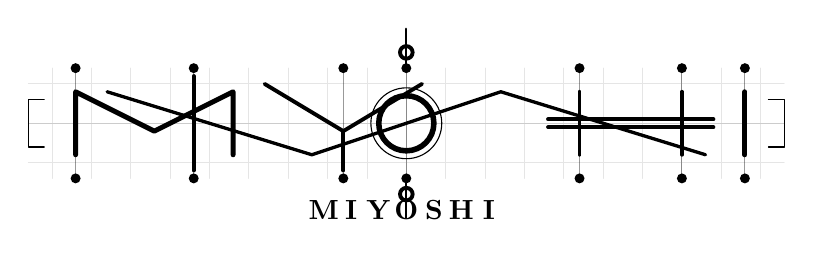
\begin{tikzpicture}[line width=1.4pt, line cap=round, line join=round]

    % --- 1. 背景の精密グリッド（高級感を出すヘアライン） ---
    \begin{scope}[gray!20, line width=0.3pt]
        \foreach \x in {-4.5, -4.0, ..., 4.5} \draw (\x, -0.7) -- (\x, 0.7);
        \draw (-4.8, 0.5) -- (4.8, 0.5);
        \draw (-4.8, -0.5) -- (4.8, -0.5);
        \draw[gray!40] (-4.8, 0) -- (4.8, 0); % 中央水平線
    \end{scope}

    % --- 2. メイン構造：MIYOSHI (幾何学構築) ---
    % M, I, Y (左)
    \draw[line width=1.8pt] (-4.2, -0.4) -- (-4.2, 0.4) -- (-3.2, -0.1) -- (-2.2, 0.4) -- (-2.2, -0.4); % M
    \draw (-2.7, -0.6) -- (-2.7, 0.6); % I (細身でスタイリッシュに)
    
    % Y, O (中央)
    \draw (-1.8, 0.5) -- (-0.8, -0.1) -- (0.2, 0.5); % YのV
    \draw (-0.8, -0.1) -- (-0.8, -0.6);             % Yの軸
    \draw[line width=2pt] (0, 0) circle (0.35);      % O (コア)
    \draw[line width=0.4pt] (0, 0) circle (0.45);    % Oの装飾外円
    
    % S (全体を貫く鋭いライン)
    \draw[line width=1.2pt] (-3.8, 0.4) -- (-1.2, -0.4) -- (1.2, 0.4) -- (3.8, -0.4);

    % H, I (右)
    \draw (2.2, -0.4) -- (2.2, 0.4);  % H左
    \draw (3.5, -0.4) -- (3.5, 0.4);  % H右
    \draw (1.8, 0.05) -- (3.9, 0.05); % H横棒
    \draw (1.8, -0.05) -- (3.9, -0.05); % H横棒 (二重線風)
    \draw[line width=1.8pt] (4.3, -0.4) -- (4.3, 0.4); % 最後のI

    % --- 3. プレミアム・ディテール装飾 ---
    
    % 各軸の端点に配置する精密ドット
    \foreach \x in {-4.2, -2.7, -0.8, 0, 2.2, 3.5, 4.3} {
        \fill[black] (\x, 0.7) circle (1.8pt);
        \fill[black] (\x, -0.7) circle (1.8pt);
        \draw[line width=0.3pt, opacity=0.4] (\x, 0.75) -- (\x, -0.75);
    }

    % 中央の垂直クロノ軸（Iの強調）
    \draw[line width=0.8pt] (0, 1.2) -- (0, 0.7);
    \draw[line width=0.8pt] (0, -1.2) -- (0, -0.7);
    \draw (0, 0.9) circle (0.08);
    \draw (0, -0.9) circle (0.08);

    % 左右の端を締めるフレーム
    \draw[line width=0.5pt] (-4.6, 0.3) -- (-4.8, 0.3) -- (-4.8, -0.3) -- (-4.6, -0.3);
    \draw[line width=0.5pt] (4.6, 0.3) -- (4.8, 0.3) -- (4.8, -0.3) -- (4.6, -0.3);

    % --- 4. サブテキスト（一文字ずつ配置してエラー回避 & 高級感） ---
    \begin{scope}[shift={(0, -1.1)}, scale=0.7]
        \node at (-1.5, 0) {\textbf{M}};
        \node at (-1.0, 0) {\textbf{I}};
        \node at (-0.5, 0) {\textbf{Y}};
        \node at (0, 0)    {\textbf{O}};
        \node at (0.5, 0)  {\textbf{S}};
        \node at (1.0, 0)  {\textbf{H}};
        \node at (1.5, 0)  {\textbf{I}};
    \end{scope}

\end{tikzpicture}
\end{document}
